%%%%%%%%%%%%%%%%%%%%%%%%
%
% $Autor: Manoj Kumar Prabhakaran $
% $Datum: 2025-03-14 $
% $Pfad: GitHub/ML24-EX03-Pico4MLPro/Pico4MLPro/Contents/General/FlashMemoryW25Q32JVSIQ.tex $
% $Version: 1 $
%
%%%%%%%%%%%%%%%%%%%%%%%%

\chapter{Flash Memory-Winbond W25Q32JVSIQ}

Our development board houses the Winbond W25Q32JVSIQ - 2246 is a 32M-bit Serial Flash memory device designed for space-constrained systems requiring efficient data storage capabilities with minimal power consumption. This NOR Flash memory component is part of Winbond's SpiFlash family, engineered specifically for applications demanding reliable code storage and execution \cite{Winbond:2016}.


\section{Hardware Interfaces}

\subsection{Serial Peripheral Interface (SPI)}
The W25Q32JVSIQ supports multiple SPI interface modes:
\begin{itemize}
	\item \textbf{Standard SPI}: Single data line (CLK, /CS, DI, DO)
	\item \textbf{Dual SPI}: Two data lines (CLK, /CS, IO0, IO1)
	\item \textbf{Quad SPI}: Four data lines (CLK, /CS, IO0, IO1, IO2, IO3) \cite{Winbond:2016}
\end{itemize}

\subsection{Pin Configuration}
The device is available in various packages with the following standard pin configurations:
\begin{itemize}
	\item \textbf{Clock (CLK)}: Provides synchronization for serial communication
	\item \textbf{Chip Select (/CS)}: Activates the device when driven LOW
	\item \textbf{Data Input/Output (DI/DO)}: Used for standard SPI operation
	\item \textbf{I/O Pins (IO0-IO3)}: Multipurpose pins for Dual/Quad SPI operation
	\item \textbf{Write Protect (/WP)}: Hardware write protection when active
	\item \textbf{Hold (/HOLD)}: Pauses device operation when active \cite{Winbond:2016}
\end{itemize}

% TikZ Diagrams for Winbond W25Q32JVSIQ Documentation

% ----------------------------------------------------------------------
% 1. Pin Configuration Diagram for 8-pin SOIC Package
% ----------------------------------------------------------------------
\begin{figure}[ht]
	\centering
	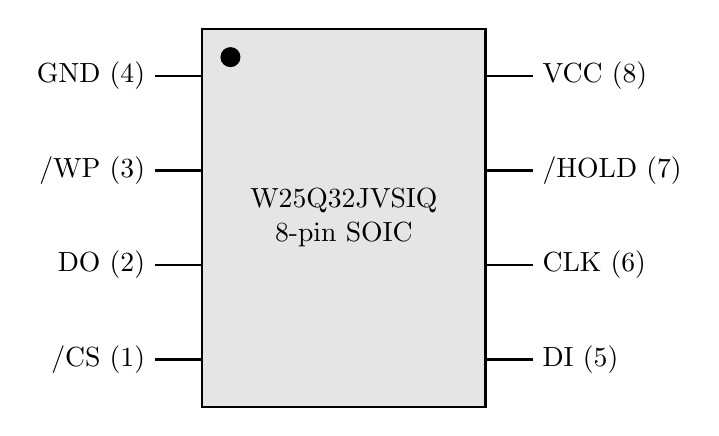
\begin{tikzpicture}[scale=1.2]
		% Draw the IC package
		\draw[thick, fill=gray!20] (0,0) rectangle (3,4);
		
		% Draw the pin 1 indicator (dot)
		\filldraw[black] (0.3,3.7) circle (0.1);
		
		% Draw pins on left side
		\foreach \y in {0.5,1.5,2.5,3.5} {
			\draw[thick] (-0.5,\y) -- (0,\y);
		}
		
		% Draw pins on right side
		\foreach \y in {0.5,1.5,2.5,3.5} {
			\draw[thick] (3,\y) -- (3.5,\y);
		}
		
		% Pin labels left side
		\node[left] at (-0.5,0.5) {/CS (1)};
		\node[left] at (-0.5,1.5) {DO (2)};
		\node[left] at (-0.5,2.5) {/WP (3)};
		\node[left] at (-0.5,3.5) {GND (4)};
		
		% Pin labels right side
		\node[right] at (3.5,3.5) {VCC (8)};
		\node[right] at (3.5,2.5) {/HOLD (7)};
		\node[right] at (3.5,1.5) {CLK (6)};
		\node[right] at (3.5,0.5) {DI (5)};
		
		% Component name
		\node[align=center] at (1.5,2) {W25Q32JVSIQ\\8-pin SOIC};
	\end{tikzpicture}
	\caption{W25Q32JVSIQ Pin Configuration (8-pin SOIC Package)}
	\label{fig:pin_config}
\end{figure}


\section{Specifications}

\subsection{Electrical Specifications}
\begin{itemize}
	\item \textbf{Operating Voltage}: 2.7V to 3.6V
	\item \textbf{Power Consumption}:
	\begin{itemize}
		\item Active Read Current: 4mA (typical)
		\item Program/Erase Current: 15mA (typical)
		\item Standby Current: 30\textmu A (typical)
		\item Power-down Current: $<$ 1\textmu A \cite{Jotrin:2018}
	\end{itemize}
\end{itemize}

\subsection{Performance Specifications}
\begin{itemize}
	\item \textbf{Clock Frequency}: Up to 133MHz for single SPI mode
	\item \textbf{Data Transfer Rate}: 66MB/s continuous
	\item \textbf{Program/Erase Cycles}: Minimum 100,000 per sector
	\item \textbf{Data Retention}: $>$20 years \cite{Jotrin:2018}
	\item \textbf{Page Program Time}: 0.7ms (typical)
	\item \textbf{Sector Erase Time}: 60ms (typical)
	\item \textbf{Block Erase Time}: 150ms (typical) \cite{Winbond:2016}
\end{itemize}

\section{Constraints}

\subsection{Operational Constraints}
\begin{itemize}
	\item \textbf{Temperature Range}: -40°C to +85°C \cite{Winbond:2024}
	\item \textbf{Maximum Junction Temperature}: 125°C
	\item \textbf{Electrostatic Discharge (ESD) Sensitivity}: 2kV (Human Body Model)
	\item \textbf{Latch-up Current}: 100mA \cite{Winbond:2016}
\end{itemize}

\subsection{Design Constraints}
\begin{itemize}
	\item \textbf{Write Protection}: Status register bits must be properly configured
	\item \textbf{Page Boundary}: Page program operations must not cross page boundaries
	\item \textbf{Erase Operations}: Memory must be erased before programming
	\item \textbf{Power Supply Stability}: Voltage must remain stable during program/erase operations \cite{Winbond:2016}
\end{itemize}

\section{Dimensions}

\subsection{Package Options and Dimensions}
\begin{itemize}
	\item \textbf{8-pin SOIC}: 208-mil width, 5.28mm × 5.20mm
	\item \textbf{8-pad WSON}: 6mm × 5mm
	\item \textbf{8-pad XSON}: 4mm × 4mm
	\item \textbf{16-pin SOIC}: 300-mil width, 10.16mm × 7.50mm
	\item \textbf{24-ball TFBGA}: 8mm × 6mm (6×4 ball array) \cite{Winbond:2024}
\end{itemize}

\subsection{Pin Spacing}
\begin{itemize}
	\item \textbf{SOIC}: 1.27mm pitch
	\item \textbf{WSON/XSON}: 0.8mm pitch
	\item \textbf{TFBGA}: 0.8mm ball pitch \cite{Winbond:2016}
\end{itemize}

\section{OS/Software Interfaces/Protocols}

\subsection{Command Protocol}
The W25Q32JVSIQ utilizes an instruction-based command protocol over the SPI interface. Key commands include:
\begin{itemize}
	\item \textbf{Read Commands}: 03h (Read Data), 0Bh (Fast Read), 3Bh (Fast Read Dual Output)
	\item \textbf{Program Commands}: 02h (Page Program), 32h (Quad Page Program)
	\item \textbf{Erase Commands}: 20h (Sector Erase), 52h (Block Erase), 60h (Chip Erase)
	\item \textbf{Status Commands}: 05h (Read Status Register), 01h (Write Status Register)
	\item \textbf{ID Commands}: 9Fh (JEDEC ID), 4Bh (Read Unique ID) \cite{Winbond:2016}
\end{itemize}

\subsection{Memory-Mapped Access}
The device supports eXecute-In-Place (XIP) functionality, allowing direct code execution from flash memory without first copying to RAM \cite{Jotrin:2018}.

\subsection{Software Driver Requirements}
\begin{itemize}
	\item Low-level SPI driver for MCU/MPU communication
	\item Flash management layer for wear leveling and bad block management
	\item File system compatibility with common embedded file systems (optional) \cite{Winbond:2016}
\end{itemize}

\section{Data}

\subsection{Data Quality}
\begin{itemize}
	\item \textbf{Error Detection}: No built-in ECC, must be implemented at system level
	\item \textbf{Security Features}:
	\begin{itemize}
		\item Software and hardware write protection mechanisms
		\item Individual block protection
		\item One-Time Programmable (OTP) security registers
		\item 64-bit unique ID for each device \cite{Winbond:2016}
	\end{itemize}
\end{itemize}

\subsection{Data Quantity}
\begin{itemize}
	\item \textbf{Total Capacity}: 32M-bit (4M-byte)
	\item \textbf{Addressable Space}: 0x000000 to 0x3FFFFF
	\item \textbf{Page Size}: 256 bytes (16,384 pages total)
	\item \textbf{Sector Size}: 4KB (1,024 sectors total)
	\item \textbf{Block Size}: 64KB (64 blocks total) \cite{Winbond:2016}
\end{itemize}

\subsection{Data Types}
\begin{itemize}
	\item \textbf{Program Data}: Code storage for microcontroller execution
	\item \textbf{Configuration Data}: System parameter storage
	\item \textbf{User Data}: Application-specific information storage
	\item \textbf{Security Data}: Storage in protected OTP security registers \cite{Jotrin:2018}
\end{itemize}

\subsection{Data Structure}
\begin{itemize}
	\item \textbf{Memory Organization}: Hierarchical structure with pages, sectors, and blocks
	\item \textbf{Address Space}: Linear addressing from 0x000000 to 0x3FFFFF
	\item \textbf{Status Registers}: Multiple status registers for device configuration
	\item \textbf{Security Registers}: Three 256-byte security registers with different access protections \cite{Winbond:2016}
\end{itemize}

\section{Code with Simple Example}

The following example demonstrates how to interface with the W25Q32JVSIQ using SPI:

\begin{lstlisting}[language=C, caption=Reading data from W25Q32JVSIQ using SPI interface]
	// Example: Reading data from W25Q32JVSIQ using SPI interface
	#include <stdio.h>
	#include "spi.h"  // MCU-specific SPI driver
	
	// W25Q32JV Command Set
	#define W25Q32_CMD_READ       0x03
	#define W25Q32_CMD_FAST_READ  0x0B
	#define W25Q32_CMD_RDID       0x9F
	#define W25Q32_CMD_WREN       0x06
	#define W25Q32_CMD_WRDI       0x04
	#define W25Q32_CMD_SE         0x20  // Sector Erase
	#define W25Q32_CMD_PP         0x02  // Page Program
	
	// SPI CS pin control (MCU-specific)
	#define W25Q32_CS_LOW()       gpio_set_level(SPI_CS_PIN, 0)
	#define W25Q32_CS_HIGH()      gpio_set_level(SPI_CS_PIN, 1)
	
	// Read Device ID
	uint32_t W25Q32_ReadID(void) {
		uint8_t buffer[3];
		uint32_t device_id;
		
		W25Q32_CS_LOW();
		
		// Send Read ID command
		spi_transfer(W25Q32_CMD_RDID);
		
		// Read 3 bytes of ID data
		buffer[0] = spi_transfer(0xFF);  // Manufacturer ID
		buffer[1] = spi_transfer(0xFF);  // Memory Type
		buffer[2] = spi_transfer(0xFF);  // Capacity
		
		W25Q32_CS_HIGH();
		
		device_id = (buffer[0] << 16) | (buffer[1] << 8) | buffer[2];
		return device_id;
	}
	
	// Read data from flash memory
	void W25Q32_Read(uint32_t address, uint8_t *data, uint32_t length) {
		W25Q32_CS_LOW();
		
		// Send Read command
		spi_transfer(W25Q32_CMD_READ);
		
		// Send 24-bit address
		spi_transfer((address >> 16) & 0xFF);
		spi_transfer((address >> 8) & 0xFF);
		spi_transfer(address & 0xFF);
		
		// Read data
		for (uint32_t i = 0; i < length; i++) {
			data[i] = spi_transfer(0xFF);
		}
		
		W25Q32_CS_HIGH();
	}
	
	// Main function example
	int main(void) {
		// Initialize SPI hardware (MCU-specific)
		spi_init();
		
		// Read and verify device ID
		uint32_t id = W25Q32_ReadID();
		printf("Device ID: 0x%06X\n", id);
		
		// Expected ID for W25Q32JVSIQ: 0xEF4016
		if (id == 0xEF4016) {
			printf("W25Q32JVSIQ detected successfully!\n");
			
			// Read first 16 bytes from flash
			uint8_t data[16];
			W25Q32_Read(0, data, 16);
			
			// Display read data
			printf("Data from address 0x000000: ");
			for (int i = 0; i < 16; i++) {
				printf("%02X ", data[i]);
			}
			printf("\n");
		} else {
			printf("Error: W25Q32JVSIQ not detected!\n");
		}
		
		return 0;
	}
\end{lstlisting}

\section{Applications}

The W25Q32JVSIQ is particularly suitable for various applications due to its high performance characteristics and low power consumption.

\subsection{Automotive Applications}
The device is designed for use in various automotive systems including:
\begin{itemize}
	\item Wireless communication systems
	\item Lidar
	\item Tire pressure detectors
	\item In-vehicle wireless charging systems
	\item Electric vehicle battery management systems
	\item Airbag systems
	\item Head-up displays
	\item Power management systems
	\item Audio systems
	\item OTA wireless systems for network communication, infotainment, and driving recorders \cite{Winbond:2024}
\end{itemize}

\subsection{Internet of Things (IoT) Applications}
The low power consumption and small form factor make the W25Q32JVSIQ ideal for IoT applications:
\begin{itemize}
	\item Code shadowing to RAM
	\item Executing code directly from Dual/Quad SPI (XIP)
	\item Storing voice, text, and data \cite{Jotrin:2018}
\end{itemize}


\clearpage